\section{Method}
\label{sec:method}

\begin{figure*}[t]
\centering
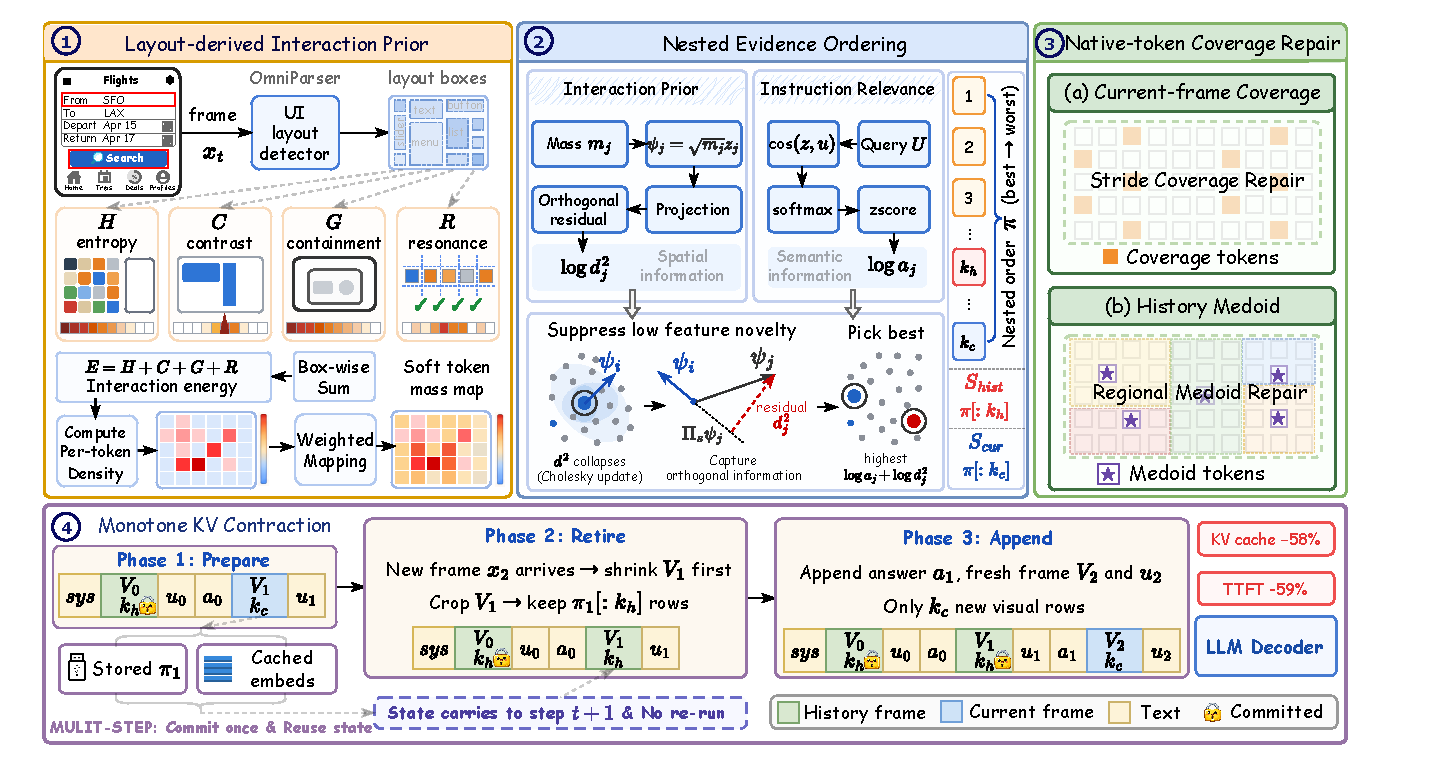
\includegraphics[width=1\linewidth]{figures/ICLR.pdf}
\vspace{-5mm}
\caption{\textbf{Overview of the proposed \method{} framework.}
\textbf{(a)~Layout-derived Interaction Prior} maps UI detections into an interaction prior.
\textbf{(b)~Nested Evidence Ordering} fuses this prior with instruction relevance and feature novelty into one nested order.
\textbf{(c)~Native-token Coverage Repair} refills the spatial gaps with native coverage and medoid tokens.
\textbf{(d)~Monotone KV Contraction} crops each retiring frame to its history prefix and restores retained rows in the next prefill.
Together, they enable trajectory-robust admission with evidence ordering for efficient GUI agents.}
\label{fig:overview}
\vspace{-2mm}
\end{figure*}

\subsection{Problem Formulation}
\label{sec:method-setup}

In multi-step GUI interaction, an agent observes a growing sequence of screenshots as an episode unfolds. 
%
At step $t$, the agent's visual encoder maps screenshot $x_t$ into $N$ raster-ordered tokens $\mathbf{E}_t\in\mathbb{R}^{N\times D}$, where $D$ is the feature dimension.
%
Under the stateless serving paradigm~\citep{li2026aquaui}, the model repeatedly prefills the current frame together with up to $H$ historical frames, which inflates both latency and memory.
%
To avoid this cost, we propose a reusable visual-state lifecycle in which each frame is encoded once and only contracts thereafter, so the retained positions must be decided before the first LLM prefill.
%
At this stage, the selector operates on the non-visual prefix $T_t$, the current visual tokens $\mathbf{E}_t$, and the admitted history, denoted collectively by $\mathcal{A}_t$.
%
For each frame $t$, let $S_t^{\mathrm{cur}}$ denote the positions retained while the frame is current, and let $S_t^{\mathrm{hist}}$ denote the smaller subset retained after retirement.
%
Formally, the reusable lifecycle imposes three constraints:
\begin{equation}
\text{(i)}\ S_t^{\mathrm{cur}}=\sigma(\mathcal{A}_t),\quad
\text{(ii)}\ S_t^{\mathrm{hist}}\subseteq S_t^{\mathrm{cur}},\quad
\text{(iii)}\ S_t^{\mathrm{cur}},S_t^{\mathrm{hist}}\subseteq\{1,\ldots,N\}.
\label{eq:lifecycle}
\end{equation}
Here, $\sigma$ denotes the selector used before prefill.
%
Condition (i) confines pruning to information available at this stage, condition (ii) enforces monotone retirement, and condition (iii) preserves original tokens to avoid synthetic merges that cannot later be dropped as cache rows.
%
These constraints make reuse realizable, yet leave open which tokens to admit while future utility remains unknown.
%
We therefore ground the evidence in the interface layout, whose operable regions are already visible.

\subsection{Layout-derived Interaction Prior}
\label{sec:method-a}
%
Relying solely on instruction relevance~\citep{zhang2025cdpruner} cannot anticipate later step demands, while uniform geometry~\citep{deng2025scope} does not separate operable regions from background.
%
To address this issue, we introduce the Layout-derived Interaction Prior (\lmp{}), which maps layout detections such as buttons and text fields into an interaction prior for the subsequent token pruning.
\\
\noindent\textbf{From Detections to Interaction Density.}
Specifically, to strengthen understanding of dense GUI screens, we detect layout boxes with OmniParser~\citep{lu2024omniparser}.
%
As illustrated by step~\cnum{1} in Fig.~\ref{fig:overview}, we compute entropy~$H$, contrast~$C$, containment~$G$ and resonance~$R$ for each box and form the interaction energy $E=H+C+G+R$.
%
Dividing by the number $n$ of active UI tokens covered by the box yields a per-token density $\rho=E/n$.
%
We then scatter $\rho$ onto the visual-token grid and max-normalize overlaps into a field $P$.
%
Then, we set $p=P/\lVert P\rVert_1$ so that only relative spatial shares enter the mapping below.
%
\noindent\textbf{From Density to Interaction Prior.}
The density $p$ marks where layout structure lies, but layout alone cannot decide admission under later steps.
%
A keep ranking from $p$ would over-commit to detections and shut out tokens that later relevance or coverage may still need.
%
We therefore turn $p$ into a soft token mass $m_j=1+\alpha Np_j$, which biases the subsequent ordering toward layout regions while keeping every token eligible.
%
Here, $\alpha\geq 0$ controls the strength of the bias, and this mass is the interaction prior passed downstream.
%
In this way, \lmp{} can inject the layout preference for the next stage to balance against instruction relevance and feature novelty.

\subsection{Nested Evidence Ordering}
\label{sec:method-b}
%
Pure relevance concentrates the budget on the strongest instruction matches~\citep{zhang2025cdpruner}, whereas diversity alone overlooks structurally important regions.
%
We therefore introduce Nested Evidence Ordering (\nwe{}), which fuses the interaction prior with instruction relevance and feature novelty into a nested order.
%
Then, every later budget can be extracted from the order's prefixes.
\\
\noindent\textbf{Relevance and Prior-weighted Features.}
Specifically, for each visual token $\mathbf e_j$, we define the normalized feature $\mathbf z_j=\mathbf e_j/\lVert\mathbf e_j\rVert_2$.
%
Besides, we normalize the instruction's token embeddings and prepend their mean to form the query matrix $\mathbf U$.
%
Then, we compute the relevance weight as follows:
\begin{equation}
    a_j =
    \mathrm{softmax}_j\!\left(
    \mathrm{zscore}\!\left(
    \max_{\mathbf u\in\mathbf U}\cos(\mathbf z_j,\mathbf u)
    \right)\right).
    \label{eq:likelihood}
\end{equation}
Here, the max keeps the strongest local match and the prepended mean anchors the score globally.
%
Besides the z-score, we also apply softmax to turn similarities into positive relative weights.
%
With the relevance in place, we next reweight each normalized feature with the interaction prior as $\boldsymbol\psi_j=\sqrt{m_j}\,\mathbf z_j$.
%
Here, layout-dense tokens matter more in the residual geometry, while the unit baseline in $m_j$ keeps every token eligible.
%
\noindent\textbf{Greedy Residual Ordering.}
To form a nested keep order, we apply the greedy relevance-weighted orthogonal residual selection with the above relevance and prior-weighted features.
%
To be specific, given a selected set $S$, it chooses the next token as follows:
\begin{equation}
j^\ast=\arg\max_{j\notin S}\bigl(\log a_j+\log d_j^2(S)\bigr),\qquad
d_j^2(S)=\lVert\boldsymbol\psi_j-\Pi_S\boldsymbol\psi_j\rVert_2^2 .
\label{eq:qd}
\end{equation}
Here, $\Pi_S$ is the orthogonal projector onto the features already in $S$.
%
With $\Psi_S=[\boldsymbol\psi_i]_{i\in S}$, we set $\Pi_S=\Psi_S(\Psi_S^{\top}\Psi_S)^{-1}\Psi_S^{\top}$ when $S$ is nonempty and $\Pi_\emptyset=\mathbf 0$.
%
The residual $d_j^2(S)$ then measures how much of $\boldsymbol\psi_j$ remains novel.
%
Adding $\log a_j$ balances that novelty against instruction relevance.
%
As illustrated by step~\cnum{2} in Fig.~\ref{fig:overview}, repeating this update produces a nested order $\pi=(\pi_1,\ldots,\pi_k)$:
\begin{equation}
S^{(k')}=\{\pi_1,\ldots,\pi_{k'}\}\subset S^{(k)}\quad\text{for }k'<k.
\label{eq:prefix}
\end{equation}
%
Retirement can therefore delete a suffix of $\pi$ rather than reselect the frame.
%
However, this order still leaves spatial placement uncontrolled.
%
A tight prefix may leave an entire region without any kept token.
%
Thus, the next stage restores the spatial coverage while preserving nesting and native tokens.

\subsection{Native-token Coverage Repair}
\label{sec:method-c}
Biased token pruning concentrates on a few strong regions and leaves other areas empty, whereas a sparse uniform lattice only partially restores the coverage~\citep{xu2026score}.
%
We therefore introduce Native-token Coverage Repair (\awc{}), which restores the spatial coverage with native tokens.
%
As shown by step~\cnum{3} in Fig.~\ref{fig:overview}, \awc{} selects different types of tokens for the current frame and history.
\\
\noindent\textbf{Current-frame Coverage Tokens.}
Specifically, the current frame uses the larger budget $k_c$, so repair can spread a few positions across the screen while keeping the strongest ordered evidence.
%
Concretely, with current dose $\rhocur\in[0,1]$, \awc{} selects $g_c=\lceil\rhocur k_c\rceil$ coverage tokens, protects the prefix $P_c=\{\pi_1,\ldots,\pi_{k_c-g_c}\}$, and takes the raster-ordered complement $U_c=(u_{(1)},\ldots,u_{(|U_c|)})$.
%
It then draws those coverage tokens from the complement by stride sampling with stride $s=\lceil|U_c|/g_c\rceil$.
%
These coverage tokens replace the unprotected tail and update $\pi$.
%
Retirement later shrinks the same frame to $k_h$, so history coverage is restored with medoid tokens rather than another stride sample.
%
\noindent\textbf{History Medoid Tokens.}
For history, with history dose $\rhohist\in[0,1]$, \awc{} sets $g_h=\lceil\rhohist k_h\rceil$ and protects a prefix of length $k_h-g_h$.
%
It then partitions the remaining space into $g_h$ near-equal regions.
%
From each region $R_b$, \awc{} keeps the medoid token $\mu_b$, which is the native token that minimizes the sum of squared feature distances to the other tokens in $R_b$.
%
The protected prefix and these medoid tokens jointly define the history subset, which stays nested inside the current keep.
%
In this way, \awc{} effectively restores spatial coverage while leaving the reusable cache realization to the next stage.

\subsection{Monotone KV Contraction}
\label{sec:method-kv}
Admission yields its advantage only if serving contracts a retired frame into the next prefill without a second visual encoding.
%
We therefore introduce Monotone KV Contraction (\kvr{}), which realizes the reusable visual-state lifecycle.
%
As illustrated by step~\cnum{4} in Fig.~\ref{fig:overview}, each step advances this state through three phases, shown here from past frame $V_0$ and current frame $V_1$.
%
\noindent\textbf{Phase 1. Prepare.}
The session holds the system prompt, past frame $V_0$ at budget $k_h$, the preceding text and answer $u_0$ and $a_0$, current frame $V_1$ at budget $k_c$, and instruction $u_1$.
%
Admission has already stored the nested order $\pi_1$ of $V_1$ and its native visual embeddings.
%
\noindent\textbf{Phase 2. Retire.}
When a new screenshot $x_2$ arrives, \kvr{} first shrinks $V_1$ before any append.
%
It truncates the cache at the boundary of $V_1$ and crops the stored embeddings to the first $k_h$ entries of $\pi_1$.
%
The operation is indexing alone and incurs no extra computation.
%
\noindent\textbf{Phase 3. Append.}
\kvr{} then restores those cropped rows with answer $a_1$, fresh frame $V_2$ and instruction $u_2$ in one merged LLM forward pass.
%
The restored rows reuse embeddings encoded when $V_1$ arrived, whereas only $V_2$ is newly encoded at budget $k_c$.
%
The resulting state leaves $V_0$ unchanged, places $V_1$ at history budget $k_h$, and makes $V_2$ the new current frame.
%
In this way, \kvr{} turns the admitted order into monotone session state.
%
It keeps the evidence native and encodes only the fresh frame at each step.
%
Overall, these components ensure efficient and robust GUI agents.
